\newpage
\chapter{Flight Test}
\label{chap:flight_test}

\section{Flight Objectives and Planning}
%write for each subsystem

For EPS: Test if suitable power could be supplied to the motors confirming plausibility of providing enough solar power for flight, test of EPS telemetry and telecommand in-flight,  

\section{Flight Results}
%write for each subsystem



\begin{figure}[H]
\centering
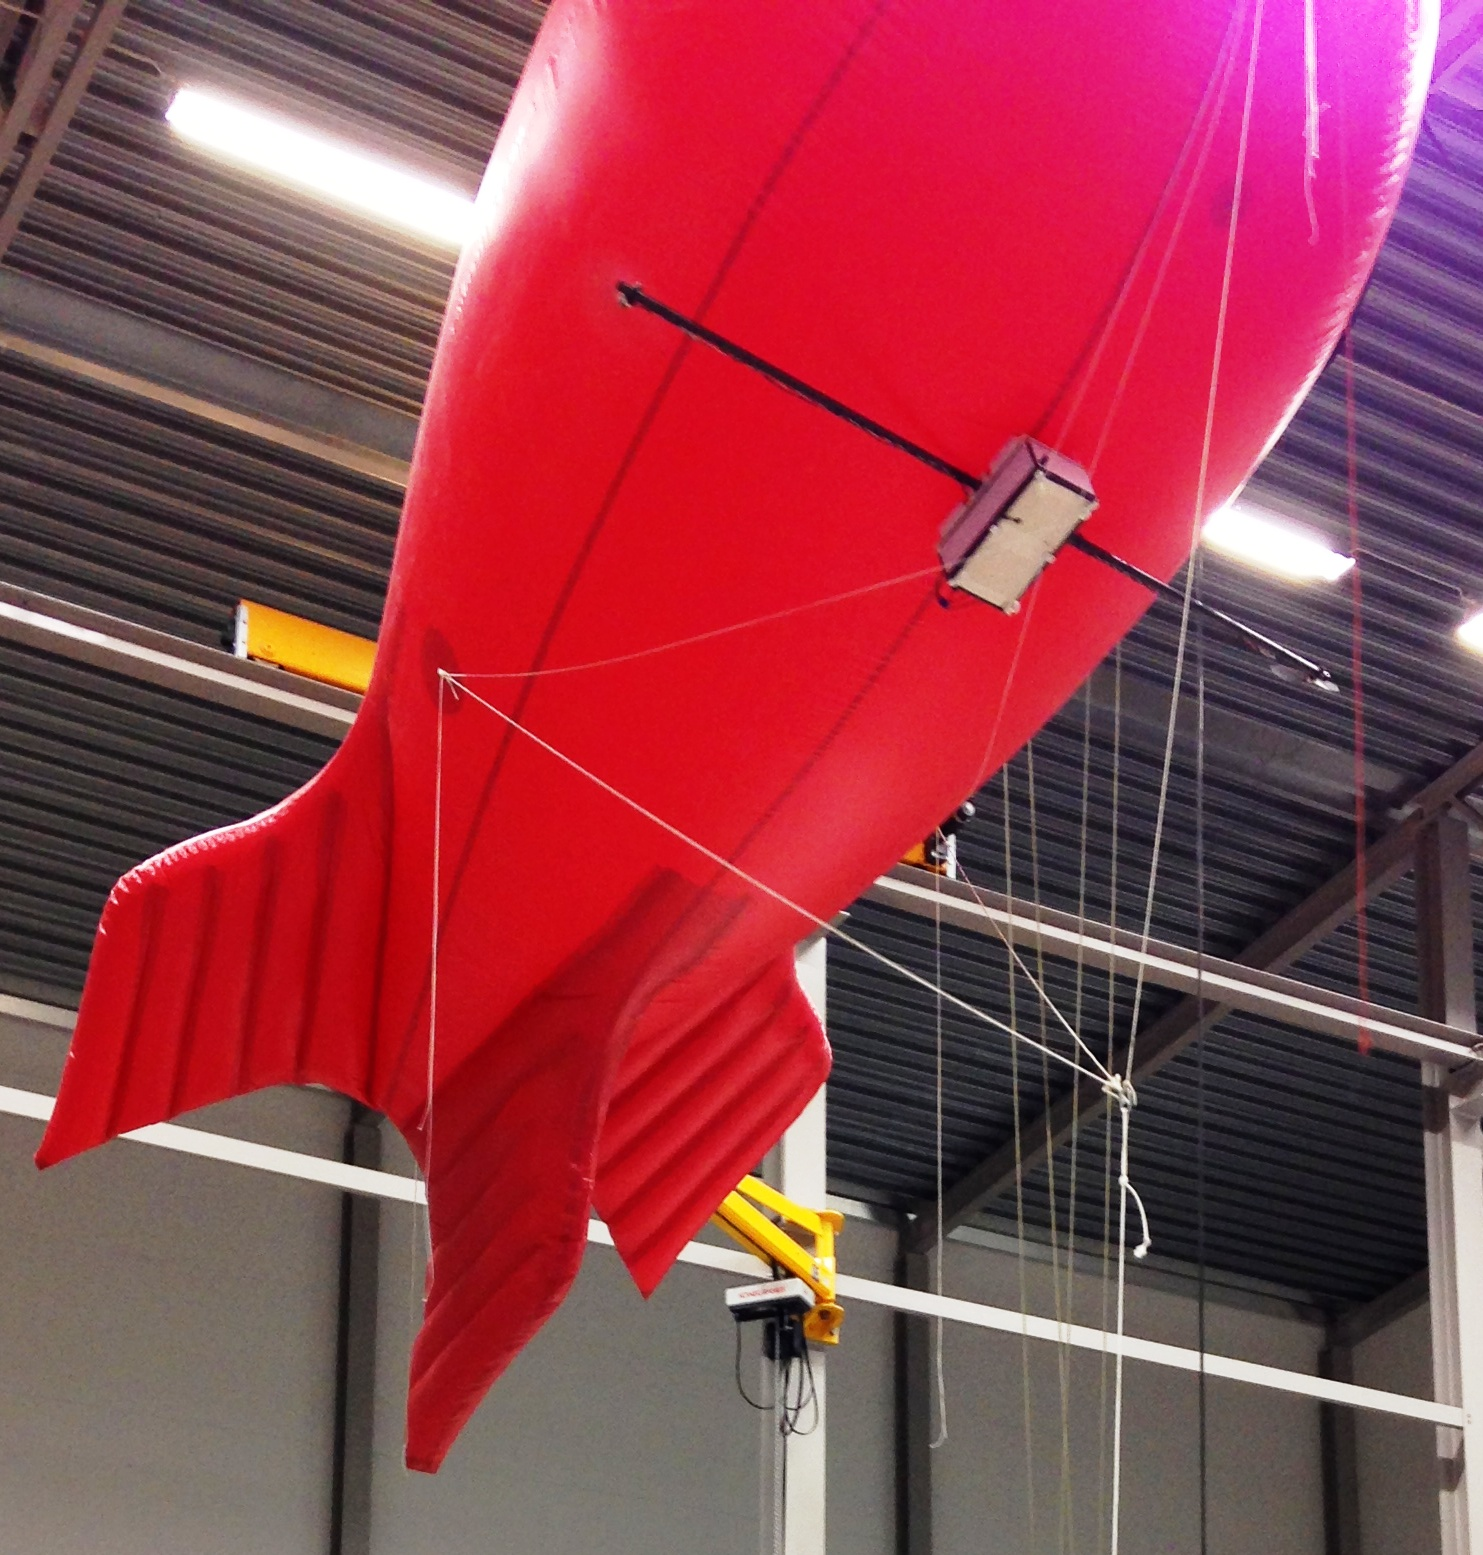
\includegraphics[width=0.7\textwidth]{figures/fig_FlightTest1_1}
\caption{First U-SPACE flight test}
\label{fig:FlightTest1_1}
\end{figure}

\begin{figure}[H]
\centering
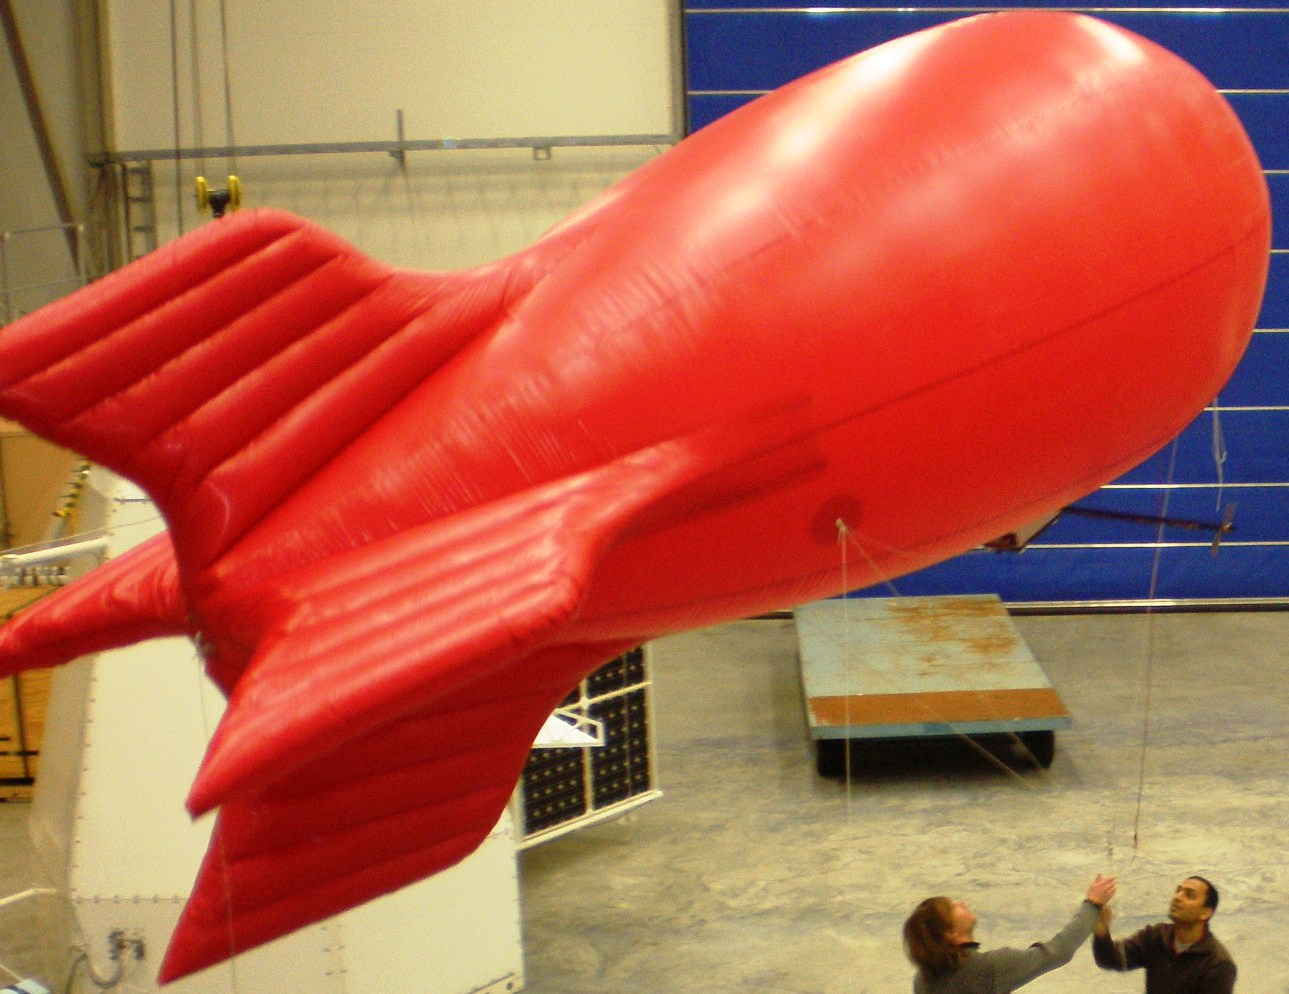
\includegraphics[width=0.7\textwidth]{figures/fig_FlightTest1_2}
\caption{First U-SPACE flight test}
\label{fig:FlightTest1_2}
\end{figure}




\section{Discussions and Future Recommendations}
%write for each subsystem
%
EPS: Due to connector issues, no telemetry was available during flight, thus detailed information of power consumption were not obtained. However, at full thrust, the system has in laboratory shown to draw around 2 x 7.5 A. At a voltage of approximately 7.0 V this corresponds to 105 W power delivered to the motors. According to \cite{website:ModelMotors}, the motors have a relatively poor efficiency of around 67\%. In \cite{CDR} the \ac{EPS} was designed to deliver minimum 40 W of continuous solar power. With these flight results, to allow continuous flight, the size of the solar array should be increased by at least a factor 2.5-3.

The BCR should be re-designed to allow higher output currents. 

A battery with higher voltage should be used - increasing power distribution efficiency and most likely also motor efficiency.